\chapter{VolWeb: La Piattaforma Web per Volatility}

L'evoluzione degli strumenti di digital forensics ha sempre seguito un percorso che bilancia potenza analitica e accessibilità. In questo contesto, VolWeb emerge come una soluzione innovativa che affronta una delle sfide più significative nell'adozione della memory forensics: la complessità d'uso degli strumenti esistenti. Sviluppato come progetto open source, VolWeb si propone di rendere le capacità avanzate di Volatility 3 accessibili attraverso un'interfaccia web moderna, eliminando molte delle barriere che tradizionalmente hanno limitato l'adozione di queste tecniche investigative.

Il presente capitolo analizza in dettaglio gli aspetti tecnici dell'implementazione, le scelte architetturali e le capacità forensi offerte dalla piattaforma nella sua versione originale.

\section{Il contesto e gli obiettivi di VolWeb}

VolWeb \cite{volweb2024} nasce dalla constatazione di un paradosso nel campo della memory forensics: mentre Volatility si è affermato come lo standard per l'analisi della memoria, le limitazioni discusse nel capitolo precedente (Sezione 2.3.3) ne hanno di fatto limitato l'adozione a una ristretta cerchia di specialisti con competenze tecniche avanzate. Questa situazione crea un collo di bottiglia operativo in molte organizzazioni, dove la capacità di analizzare rapidamente dump di memoria può fare la differenza tra contenere un incidente o subirne le conseguenze complete.

Il progetto, avviato nel 2023, si inserisce in un momento storico particolare per la cybersecurity. L'aumento esponenziale degli attacchi ransomware, la sofisticazione crescente delle Advanced Persistent Threats e l'adozione massiva del lavoro remoto hanno moltiplicato la superficie di attacco delle organizzazioni. In questo scenario, la capacità di condurre analisi forensi rapide ed efficaci diventa non più un lusso per pochi specialisti, ma una necessità operativa diffusa.

In risposta a queste sfide, VolWeb persegue tre obiettivi fondamentali strettamente interconnessi. Il primo è la democratizzazione dell'accesso alle capacità di memory forensics attraverso un'interfaccia che nasconda la complessità di Volatility senza sacrificarne la potenza. Questo obiettivo si concretizza nella riduzione del tempo necessario per ottenere risultati actionable da ore a minuti, permettendo anche ad analisti con esperienza limitata di condurre investigazioni efficaci. 

Il secondo obiettivo riguarda la standardizzazione dei workflow investigativi. Mentre l'uso diretto di Volatility lascia ampia libertà nell'approccio all'analisi, questa flessibilità può tradursi in inconsistenza e inefficienza, specialmente in team con membri di diversa esperienza. VolWeb introduce quindi un framework strutturato che guida l'analista attraverso le fasi dell'investigazione, garantendo completezza e riproducibilità. 

Il terzo pilastro è rappresentato dalla collaborazione, essenziale nelle investigazioni moderne che raramente coinvolgono un singolo analista ma richiedono il coordinamento di team distribuiti geograficamente e temporalmente. VolWeb fornisce un ambiente condiviso dove più analisti possono lavorare sugli stessi casi, condividere osservazioni e costruire collettivamente la comprensione di un incidente.


\section{Principi architetturali}

L'architettura di VolWeb riflette una filosofia di design che privilegia modularità, estensibilità e manutenibilità. La scelta di un'architettura web-based deriva da considerazioni pratiche sull'uso reale dello strumento in contesti operativi. Gli analisti forensi operano spesso in condizioni di emergenza, da postazioni diverse e con risorse hardware variabili. Un'applicazione web elimina le frizioni legate all'installazione e configurazione di software complesso, permettendo un accesso immediato alle funzionalità di analisi.

La separazione tra frontend e backend attraverso API REST \cite{restapi} rappresenta una scelta architettonica fondamentale che va oltre la semplice modularizzazione del codice. Questa separazione permette l'evoluzione indipendente dei componenti, facilitando sia lo sviluppo che la manutenzione. Inoltre, esporre le funzionalità attraverso API standardizzate apre la possibilità di integrazioni con altri strumenti dell'ecosistema di sicurezza, trasformando VolWeb da applicazione standalone a componente di pipeline di analisi più ampie.

\subsection{Stack tecnologico}

\begin{figure}[H]
    \centering
    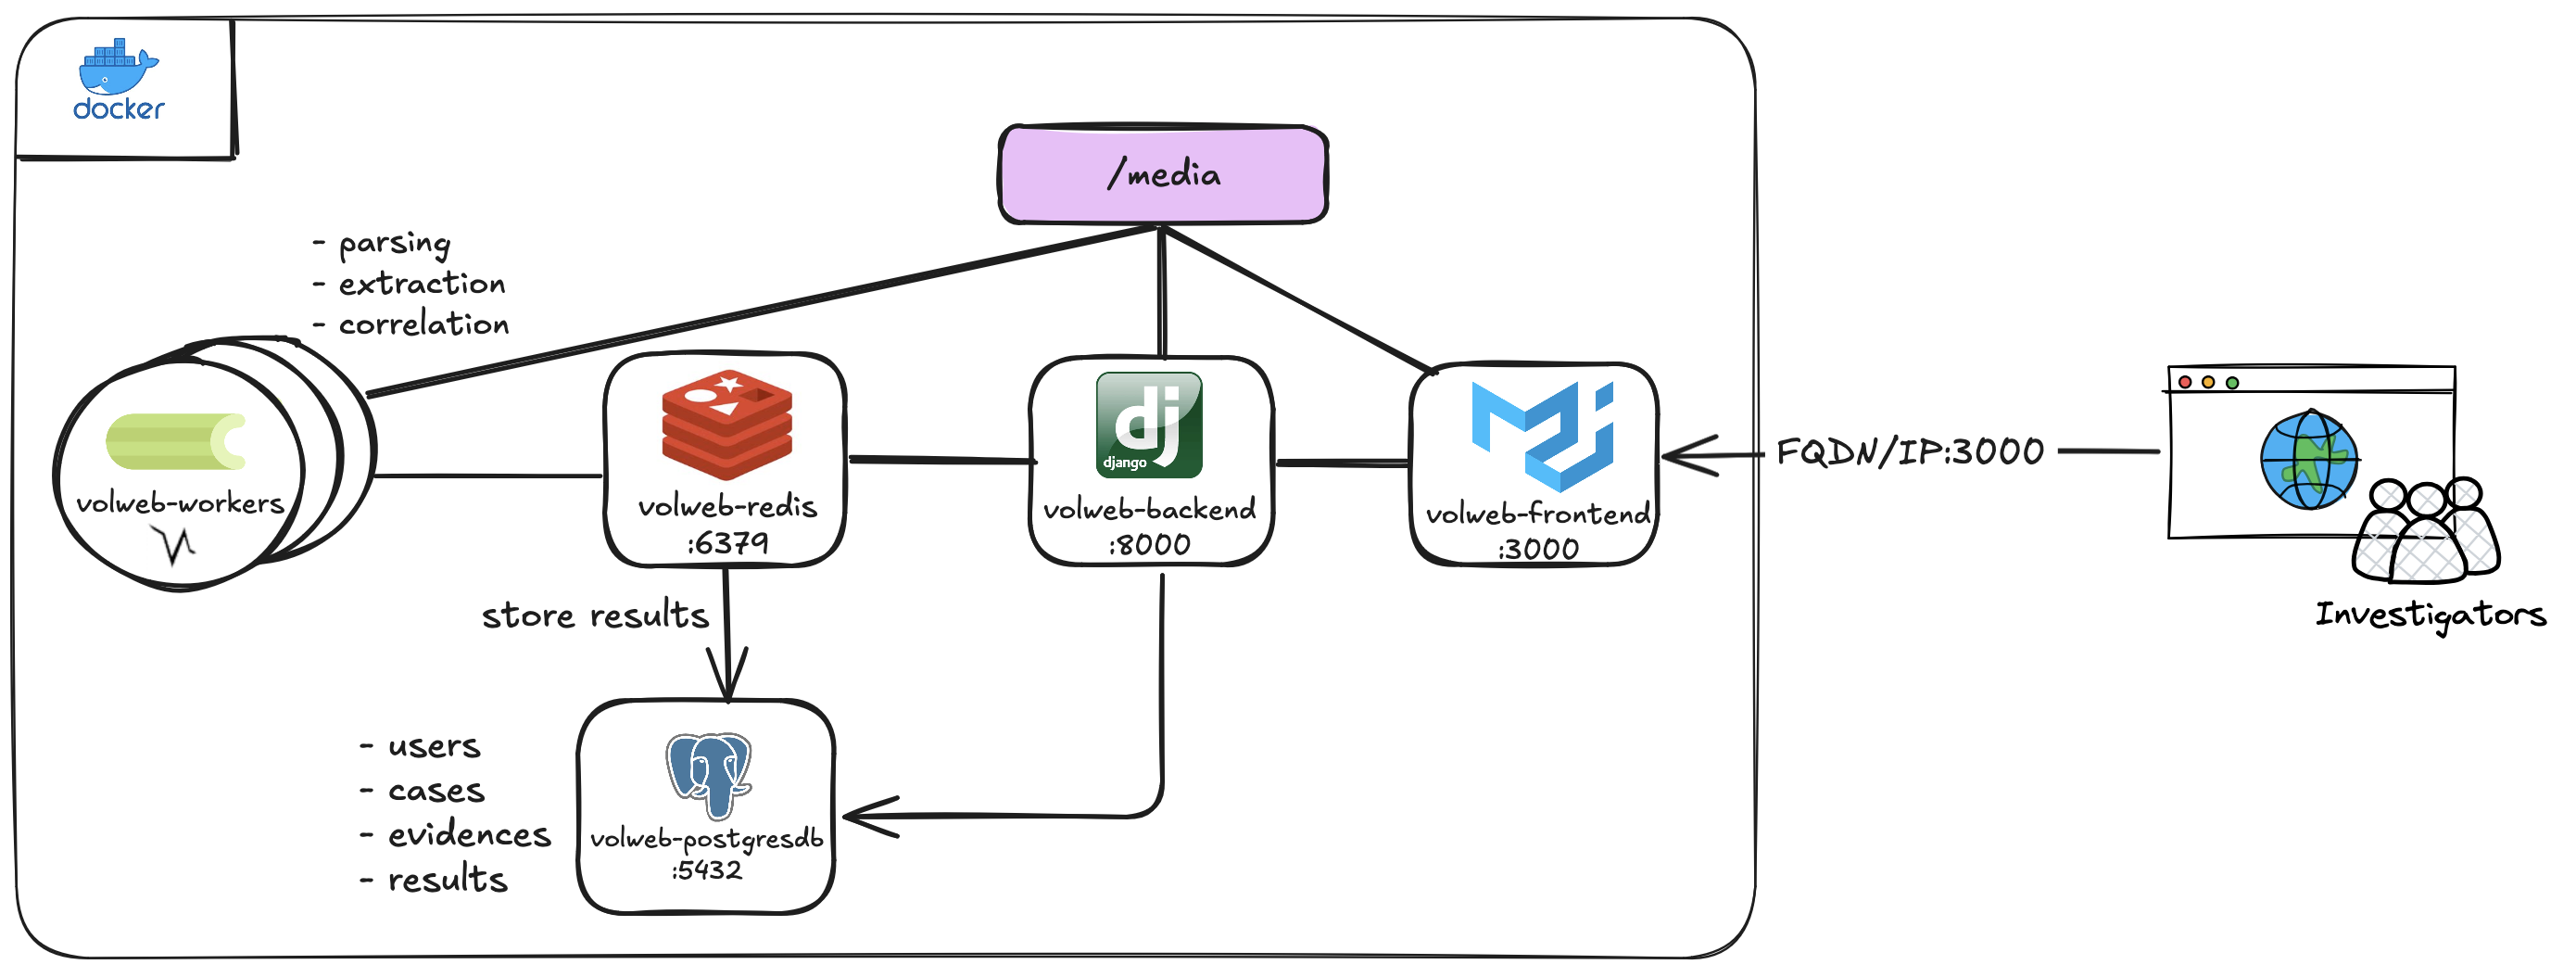
\includegraphics[width=1\linewidth]{images/volweb-original/volweb-arch.png}
\end{figure}

La selezione delle tecnologie utilizzate in VolWeb riflette un bilanciamento tra maturità, performance e facilità di sviluppo. Il backend, costruito su \textbf{Django 4.2} e \textbf{Django REST Framework}, sfrutta un ecosistema consolidato che offre soluzioni robuste per problematiche comuni come autenticazione, gestione delle sessioni e validazione dei dati. La scelta di Django non è casuale: il framework Python si integra naturalmente con Volatility 3, permettendo un'interazione diretta senza layer di traduzione aggiuntivi.

Il frontend utilizza \textbf{React 18.2.0} con \textbf{Material-UI 5.14} per l'interfaccia utente. Questa combinazione fornisce un'esperienza utente moderna e reattiva, fondamentale per mantenere l'efficienza operativa durante investigazioni che possono protrarsi per ore. La scelta di Material-UI come design system garantisce consistenza visiva e accessibilità, aspetti spesso trascurati nei tool forensi ma cruciali per ridurre il carico cognitivo dell'analista durante sessioni di analisi intensive.

Per la gestione dei task asincroni, VolWeb si affida a \textbf{Celery 5.3} con \textbf{Redis} come message broker. Questa architettura permette di gestire operazioni computazionalmente intensive come l'analisi di dump di memoria di grandi dimensioni senza bloccare l'interfaccia utente. La scalabilità orizzontale offerta da Celery consente inoltre di distribuire il carico di lavoro su molteplici macchine, aspetto critico quando si devono analizzare contemporaneamente dump provenienti da decine di endpoint compromessi.

La persistenza dei dati è affidata a \textbf{PostgreSQL}, scelto per la sua affidabilità e le capacità avanzate di gestione di dati JSON, particolarmente utili per memorizzare i risultati strutturati ma eterogenei prodotti dai vari plugin di Volatility. L'uso di SQLite come alternativa per deployment di sviluppo o di piccola scala dimostra l'attenzione alla flessibilità di deployment, permettendo agli sviluppatori di avere un ambiente funzionale senza la complessità di configurare un database server completo.

\subsection{Integrazione con Volatility 3}

Il cuore tecnico di VolWeb risiede nell'integrazione con Volatility 3, realizzata attraverso un layer di astrazione che gestisce la complessità dell'interazione con il framework. Questa integrazione non si limita a un semplice wrapper delle funzionalità command-line, ma implementa una gestione sofisticata del ciclo di vita dell'analisi.

Il modulo definito in 'backend/volatility\_engine.py' implementa un'interfaccia Python nativa con Volatility 3. Questo approccio elimina l'overhead dell'invocazione di processi esterni e permette un controllo granulare sull'esecuzione dei plugin. La gestione della configurazione di Volatility, tradizionalmente complessa e error-prone, viene automatizzata attraverso la costruzione dinamica del contesto di esecuzione basata sui metadati del dump analizzato.

Un aspetto particolarmente innovativo dell'integrazione riguarda la gestione dei simboli. Volatility richiede symbol tables specifiche per ogni versione di sistema operativo per interpretare correttamente le strutture dati in memoria. VolWeb automatizza il download e la gestione di questi simboli, eliminando uno dei principali ostacoli tecnici nell'uso di Volatility. Il sistema mantiene una cache locale dei simboli più comuni e scarica automaticamente quelli mancanti quando necessario. Inoltre, permette anche di caricare manualmente i file dei simboli direttamente dal file system, offrendo all'utente un controllo completo in caso di configurazioni particolari o ambienti offline.

La gestione degli errori rappresenta un altro aspetto critico dell'integrazione. I plugin di Volatility possono fallire per molteplici ragioni, dalla corruzione del dump all'incompatibilità con la versione del sistema operativo. VolWeb implementa una strategia di error handling che distingue tra errori fatali e warning, permettendo all'analisi di procedere anche quando singoli plugin falliscono, mentre registra dettagliatamente le cause del fallimento per troubleshooting successivo.

\subsection{Requisiti di sistema e installazione}

Prima di procedere con l'installazione di VolWeb, è necessario verificare che l'ambiente soddisfi i requisiti minimi. Il sistema richiede \textbf{Python 3.8 o superiore}, fondamentale per la compatibilità con Volatility 3 e le librerie moderne utilizzate. È inoltre necessario avere Git installato per clonare il repository e Docker con Docker Compose per il deployment containerizzato, che rappresenta il metodo di installazione raccomandato.

Dal punto di vista hardware, sebbene VolWeb possa funzionare su sistemi modesti per analisi di piccola scala, per un utilizzo produttivo si raccomandano almeno 8 GB di RAM e storage sufficiente per i dump di memoria, che possono facilmente raggiungere decine di gigabyte per sistema analizzato. La disponibilità di CPU multi-core è fortemente raccomandata per sfruttare appieno le capacità di elaborazione parallela offerte da Celery.

L'installazione di VolWeb è stata progettata per essere il più semplice possibile, riconoscendo che la complessità di setup è spesso una barriera all'adozione. Il processo standard prevede prima di tutto la clonazione del repository:

\begin{minted}[bgcolor=gray!10, fontsize=\small]{bash}
git clone https://github.com/k1nd0ne/VolWeb.git
cd VolWeb
\end{minted}

Successivamente, l'ambiente può essere avviato utilizzando Docker Compose, che gestisce automaticamente tutte le dipendenze e configurazioni:

\begin{minted}[bgcolor=gray!10, fontsize=\small]{bash}
docker-compose up -d
\end{minted}

La containerizzazione offre vantaggi significativi per la riproducibilità e la portabilità, garantendo che gli stessi container possano essere deployati in ambiente di sviluppo, test e produzione con comportamento consistente.

\section{Workflow Operativo e Gestione}

\subsection{Gestione dei casi}

Il workflow operativo di VolWeb inizia con la creazione di un caso, che rappresenta il contenitore logico per un'investigazione. Ogni caso può aggregare molteplici evidenze, permettendo l'analisi correlata di dump provenienti da sistemi diversi coinvolti nello stesso incidente. La gestione dei casi segue best practice forensi, mantenendo metadati completi su chi ha creato il caso, quando è stato modificato e quale sia il suo stato corrente.

\begin{figure}[H]
    \centering
    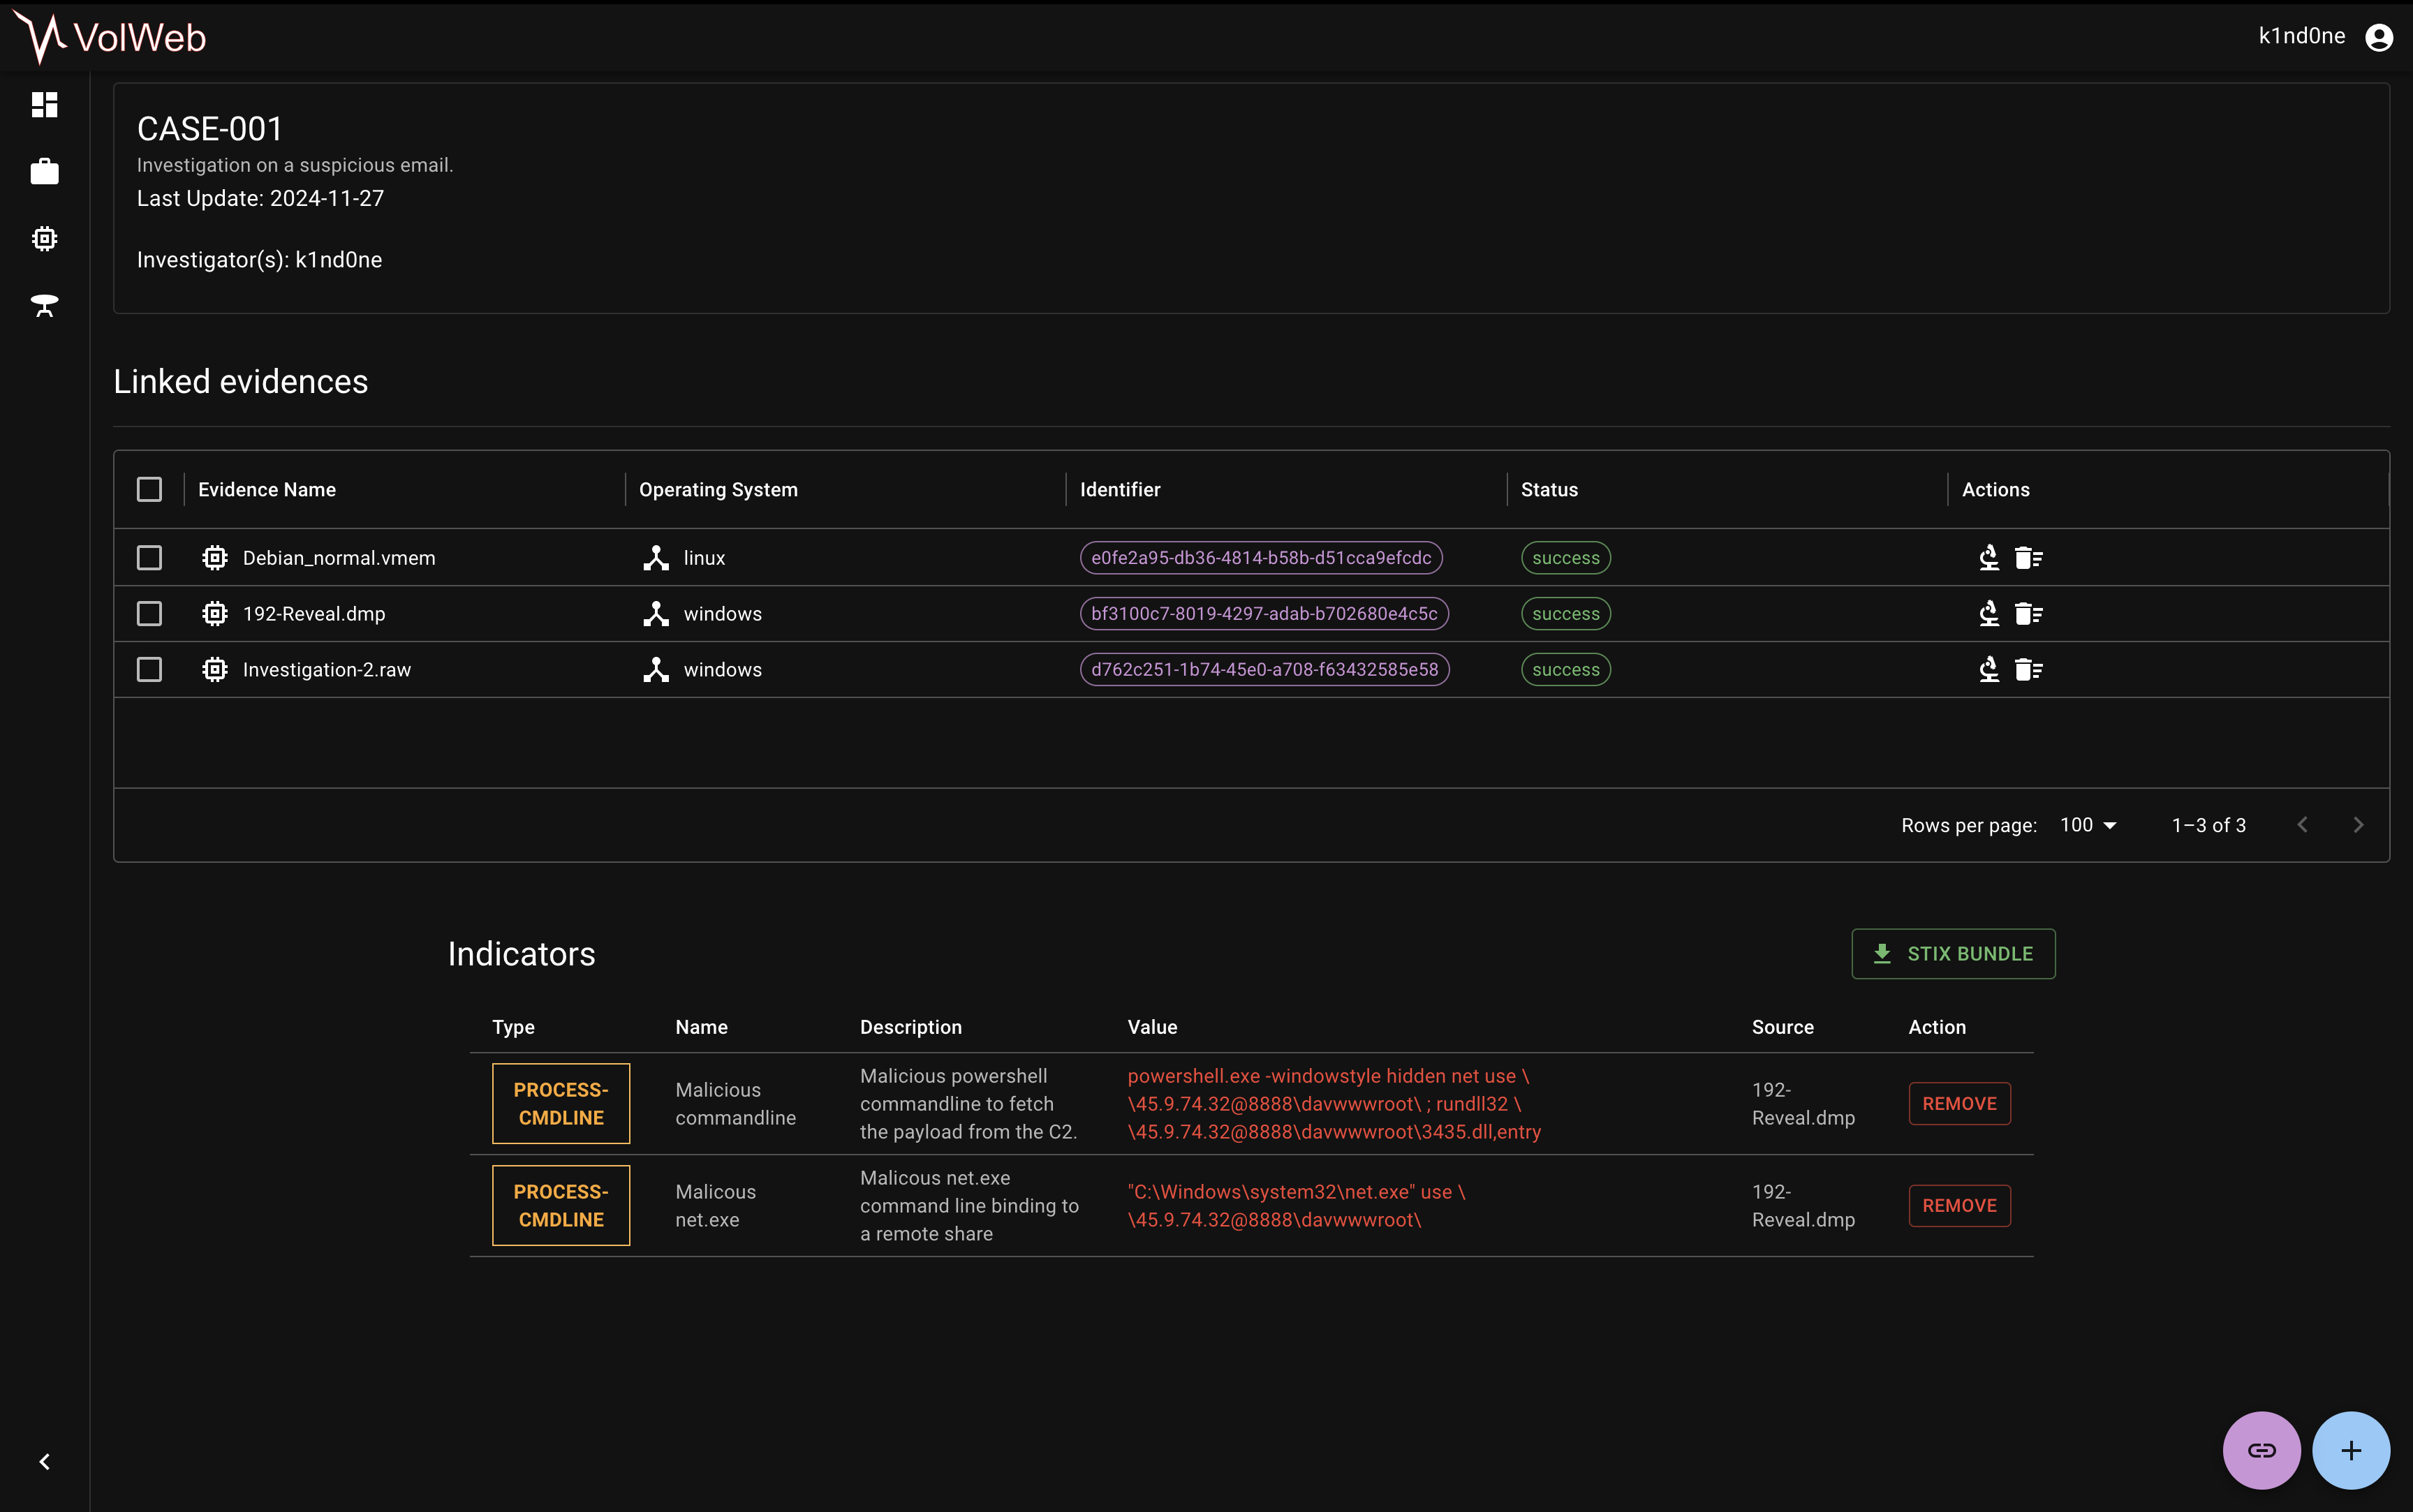
\includegraphics[width=1\linewidth]{images/volweb-original/volweb-case-management.png}
\end{figure}

L'interfaccia di gestione presenta una dashboard che fornisce una vista immediata dello stato delle investigazioni. Ogni caso è rappresentato da una card che mostra informazioni essenziali: nome, descrizione, numero di evidenze associate, stato dell'analisi e ultima modifica. Questa presentazione visiva permette agli analisti di prioritizzare rapidamente il proprio lavoro e identificare casi che richiedono attenzione immediata.

\subsection{Upload e Gestione dei Dump di Memoria}

Una volta creato un caso, il passo successivo è l'upload dei dump di memoria da analizzare. VolWeb gestisce questo processo critico con particolare attenzione all'integrità dei dati e all'esperienza utente. L'interfaccia di upload supporta drag-and-drop, permettendo agli utenti di trascinare file direttamente dal file manager del sistema operativo.

\begin{figure}[H]
    \centering
    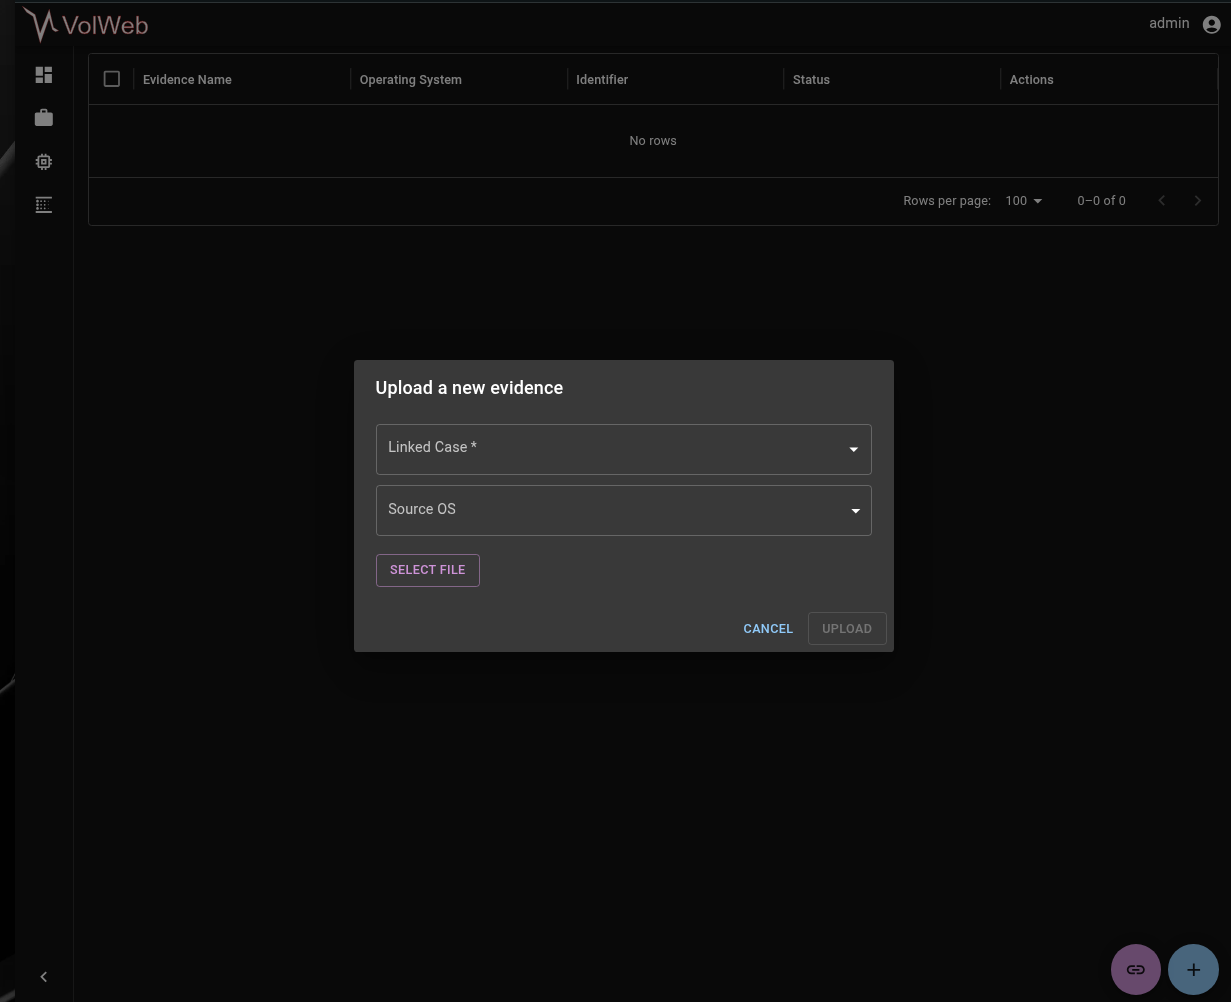
\includegraphics[width=0.9\linewidth]{images/volweb-original/volweb-upload-interface.png}
\end{figure}

La gestione di file di grandi dimensioni rappresenta una sfida tecnica significativa in un'applicazione web. I dump di memoria possono facilmente superare i 10 GB, dimensioni che mettono alla prova sia l'infrastruttura di rete che i meccanismi standard di upload HTTP. VolWeb affronta questa sfida attraverso un sistema sofisticato di gestione che combina upload chunked, validazione dell'integrità e rilevamento automatico del profilo.

Per file di grandi dimensioni, comune scenario con dump di memoria che possono superare i 16GB, VolWeb implementa un sistema di upload chunked. Questo approccio divide il file in blocchi più piccoli che vengono trasmessi sequenzialmente, con la possibilità di riprendere l'upload in caso di interruzione della connessione. Il backend gestisce l'assemblaggio dei chunk e la validazione dell'integrità attraverso hash crittografici, mantenendo metadati dettagliati su ogni file inclusi hash multipli per la verifica dell'integrità e timestamp per la chain of custody.

Uno degli aspetti più innovativi di VolWeb è il sistema di rilevamento automatico del profilo del sistema operativo. Questo processo, tradizionalmente manuale e soggetto a errori, viene automatizzato attraverso l'analisi delle strutture dati presenti nel dump. Il sistema esamina prima signature ad alta confidenza che permettono l'identificazione immediata. Se queste non producono risultati, procede con euristiche più complesse che analizzano pattern di strutture dati. Come fallback finale, l'utente può specificare manualmente il profilo, ma nella pratica questo è raramente necessario.

\subsection{Analisi automatica}

Dopo il completamento dell'upload, VolWeb avvia automaticamente una serie di analisi predefinite progettate per fornire una panoramica immediata del sistema analizzato. Questa suite di plugin include l'enumerazione dei processi attraverso \textbf{pslist}, l'analisi delle connessioni di rete con \textbf{netscan}, l'estrazione delle command line tramite \textbf{cmdline}, la lista delle DLL caricate utilizzando \textbf{dlllist} e l'identificazione degli handle aperti con \textbf{handles}.

La selezione di questi plugin non è casuale ma deriva dall'esperienza operativa che identifica queste informazioni come il minimo dataset necessario per una comprensione iniziale dello stato del sistema. L'esecuzione automatica elimina la necessità per l'analista di ricordare quali plugin eseguire per primi, standardizzando l'approccio investigativo.

Durante l'analisi, VolWeb fornisce feedback dettagliato attraverso WebSocket, mostrando quale plugin è in esecuzione, la percentuale di completamento e eventuali warning o errori. Questo feedback real-time è cruciale per mantenere la fiducia dell'utente durante operazioni che possono richiedere tempo significativo.

\section{Interfaccia Utente e Visualizzazioni}

\subsection{Design dell'interfaccia}

L'interfaccia di VolWeb rappresenta un departure significativo dall'approccio command-line tradizionale di Volatility. Il design, basato sui principi del Material Design, prioritizza la chiarezza e l'efficienza operativa. La dashboard principale presenta una vista d'insieme dei casi attivi, permettendo all'analista di comprendere immediatamente lo stato delle investigazioni in corso.

\begin{figure}[H]
    \centering
    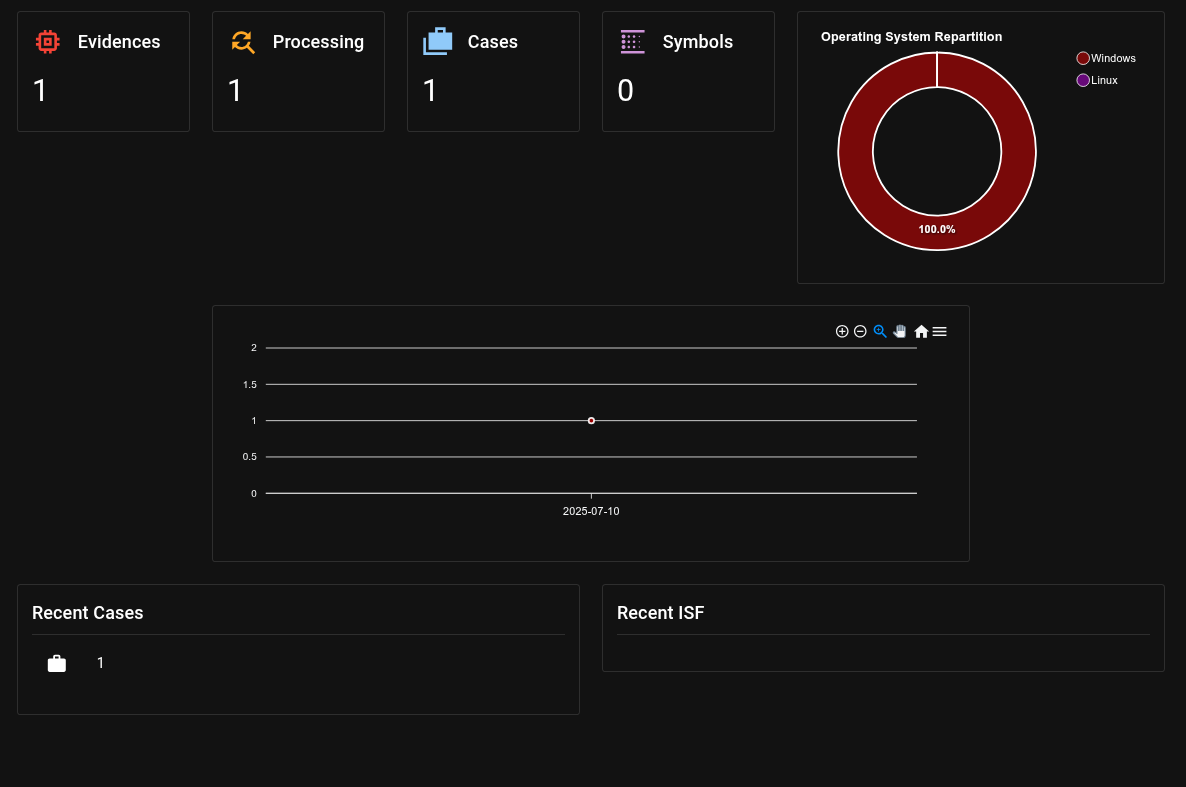
\includegraphics[width=1\linewidth]{images/volweb-original/volweb-dashboard.png}
\end{figure}

La navigazione segue una struttura gerarchica naturale: dalla lista dei casi si accede ai dettagli del singolo caso, da cui è possibile esplorare le evidenze associate e i risultati delle analisi. Questa struttura, apparentemente semplice, nasconde una considerevole complessità nell'orchestrazione dei componenti React che gestiscono lo stato dell'applicazione.

L'uso estensivo di feedback visivo mantiene l'utente informato sullo stato delle operazioni. Progress bar per upload e analisi, notifiche per il completamento di task e indicatori di stato per ogni componente contribuiscono a creare un'esperienza utente che minimizza l'incertezza e l'ansia tipiche delle operazioni di lunga durata.

\subsection{Visualizzazione dei risultati}

La presentazione efficace dei risultati rappresenta uno dei maggiori valori aggiunti di VolWeb rispetto all'uso diretto di Volatility. Invece di output testuali densi, VolWeb trasforma i dati in visualizzazioni interattive che facilitano l'identificazione di anomalie e pattern sospetti.

La presentazione dei risultati dell'analisi rappresenta una delle sfide principali nel design di VolWeb. I plugin di Volatility producono output eterogenei, da semplici liste a strutture dati complesse. VolWeb implementa renderer specializzati per i tipi di dati più comuni, trasformando tabelle di testo in visualizzazioni interattive.

\subsubsection{Visualizzazione dei processi}

La vista dei processi utilizza una rappresentazione ad albero che mostra chiaramente le relazioni parent-child tra processi. I processi orfani o con parent inusuali sono evidenziati visualmente, permettendo l'identificazione rapida di potenziali indicatori di compromissione. Ogni nodo dell'albero è espandibile per rivelare dettagli aggiuntivi come PID, tempo di creazione, numero di thread e handle, e spazio di memoria utilizzato.

\begin{figure}[H]
    \centering
    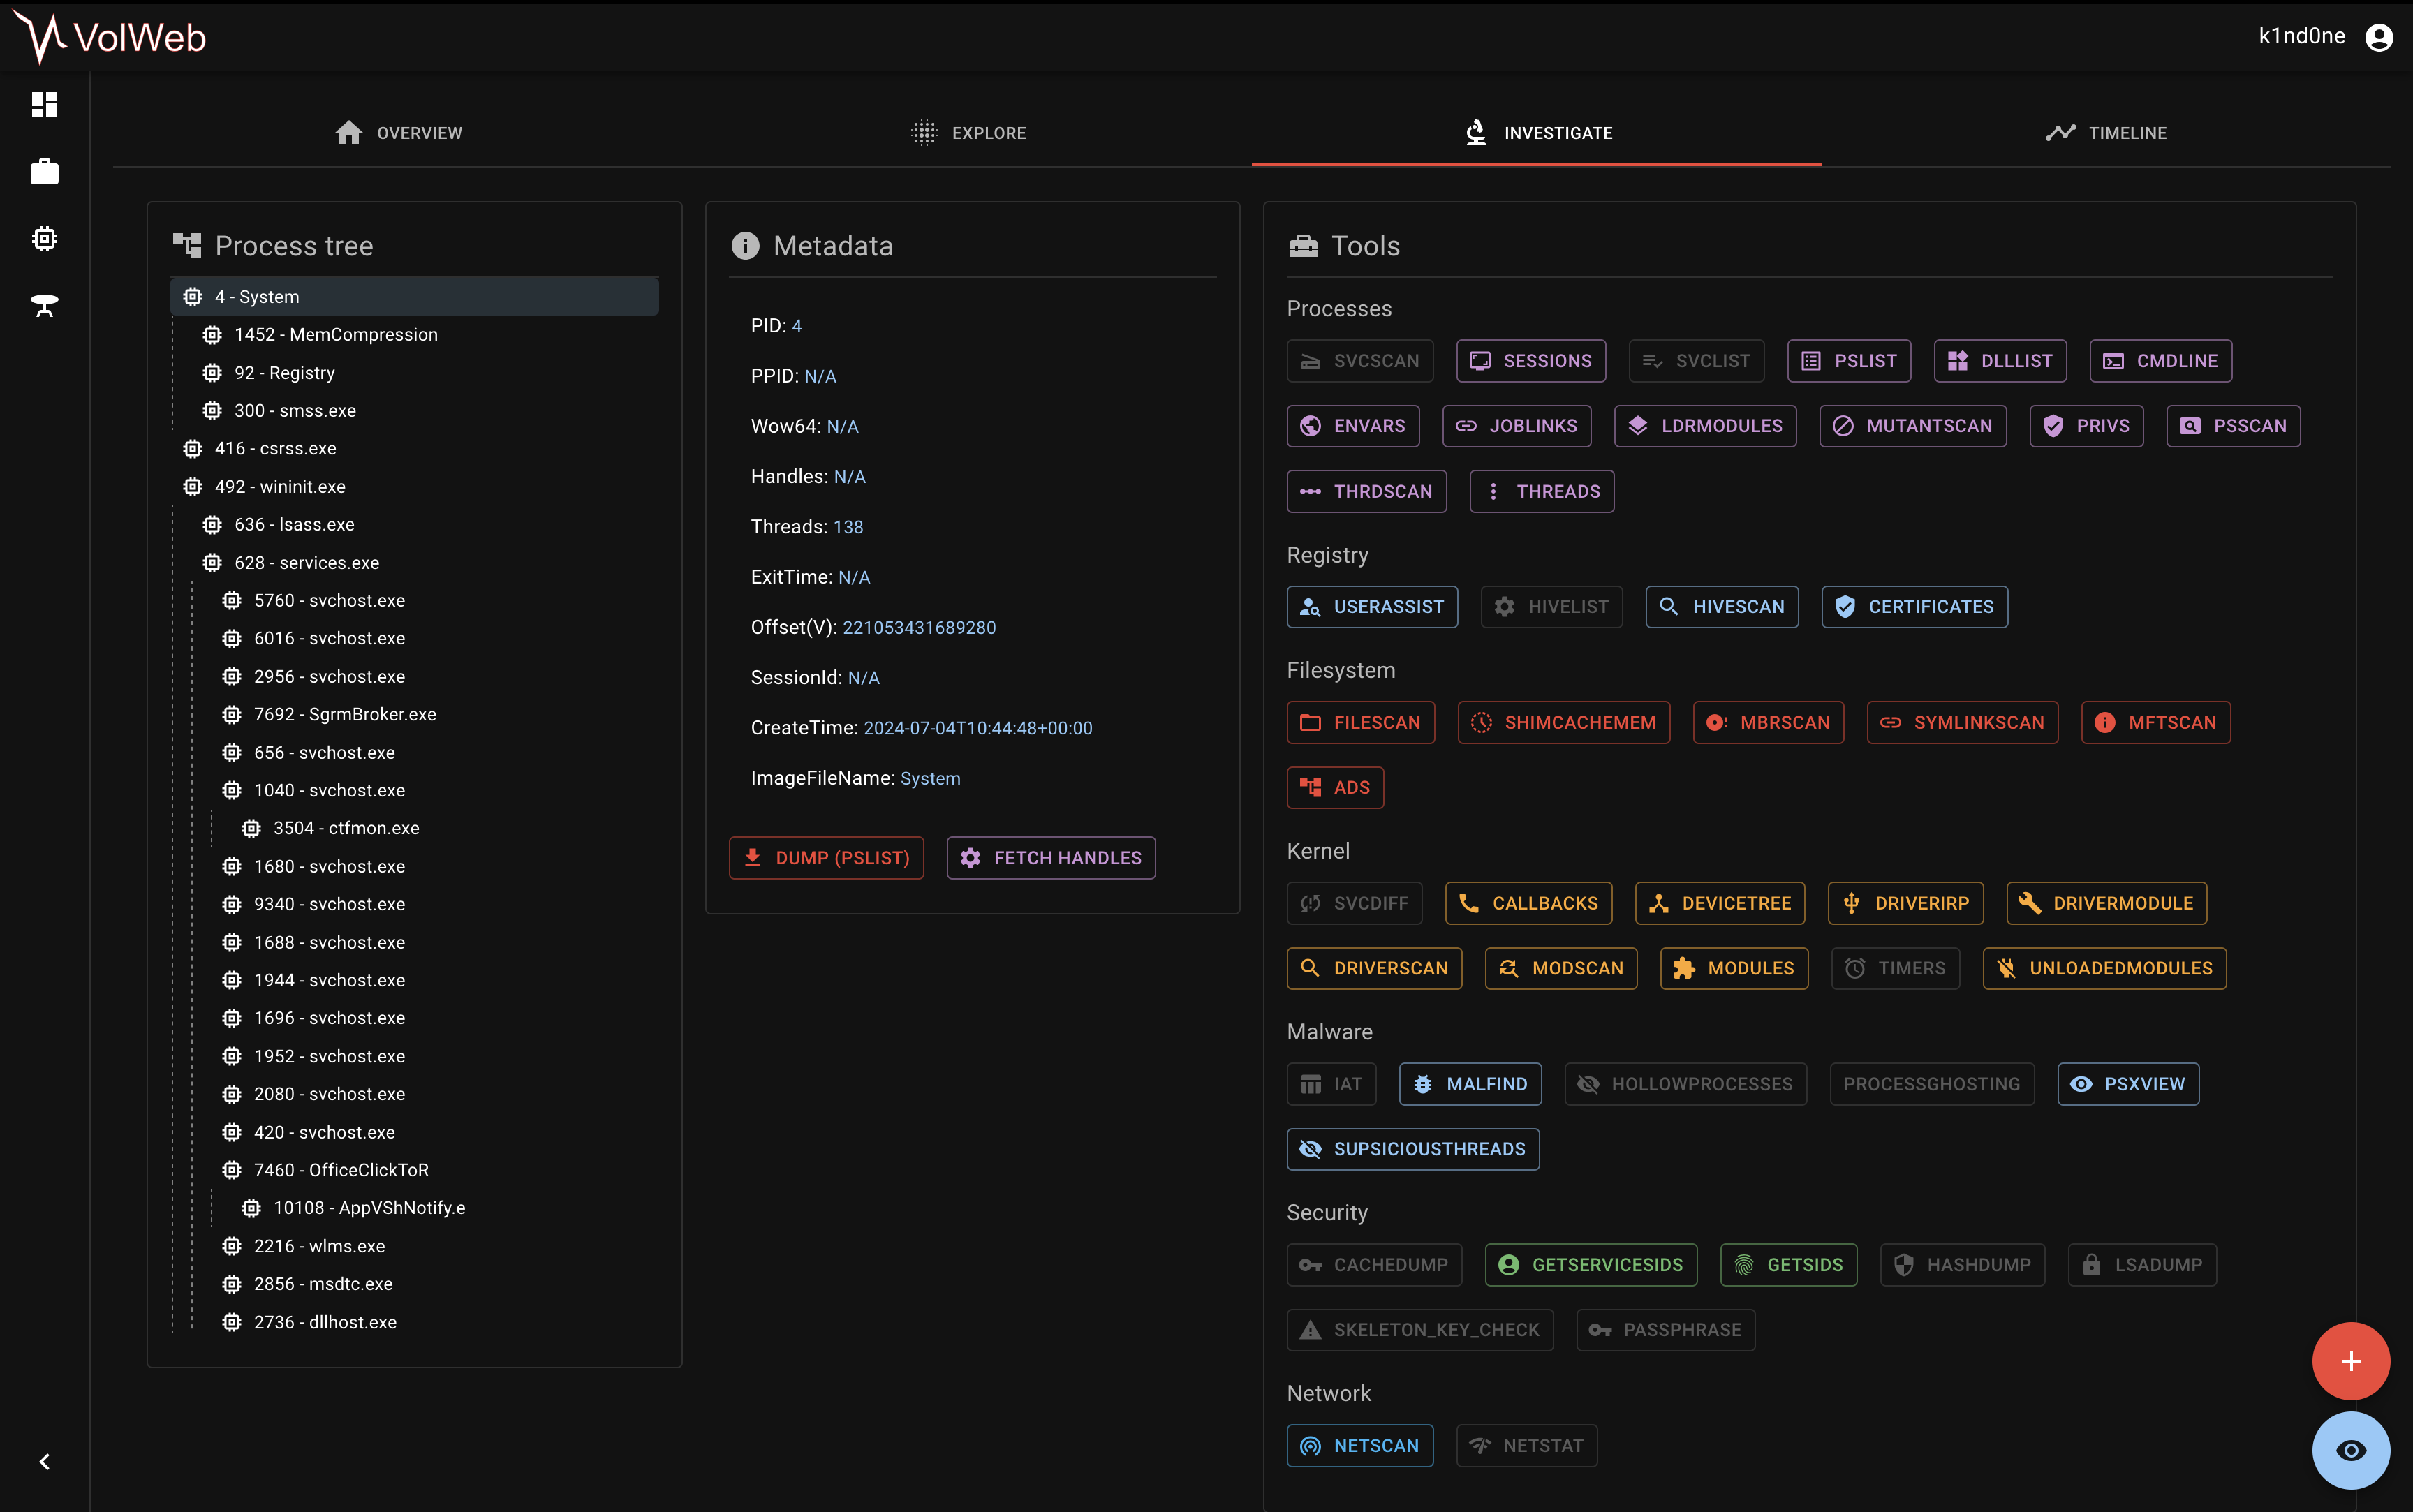
\includegraphics[width=1\linewidth]{images/volweb-original/volweb-process-tree.png}
\end{figure}

Per i dati di processo, il sistema presenta una vista tabellare arricchita che permette sorting, filtering e ricerca full-text. Ogni processo è cliccabile per accedere a una vista dettagliata che aggrega informazioni da multipli plugin correlati. Questa aggregazione, invisibile all'utente, richiede una logica complessa per correlare dati provenienti da plugin diversi basandosi su identificatori comuni come PID e offset di memoria.

\subsubsection{Visualizzazione delle connessioni di rete}

Per le connessioni di rete, VolWeb offre multiple viste complementari. La vista tabellare fornisce tutti i dettagli tecnici: processo proprietario, protocollo, indirizzi IP e porte locali e remote, stato della connessione. La vista grafica, basata su D3.js, visualizza le connessioni come un grafo interattivo dove i nodi rappresentano processi ed endpoint, mentre gli archi indicano le connessioni attive.

\begin{figure}[H]
    \centering
    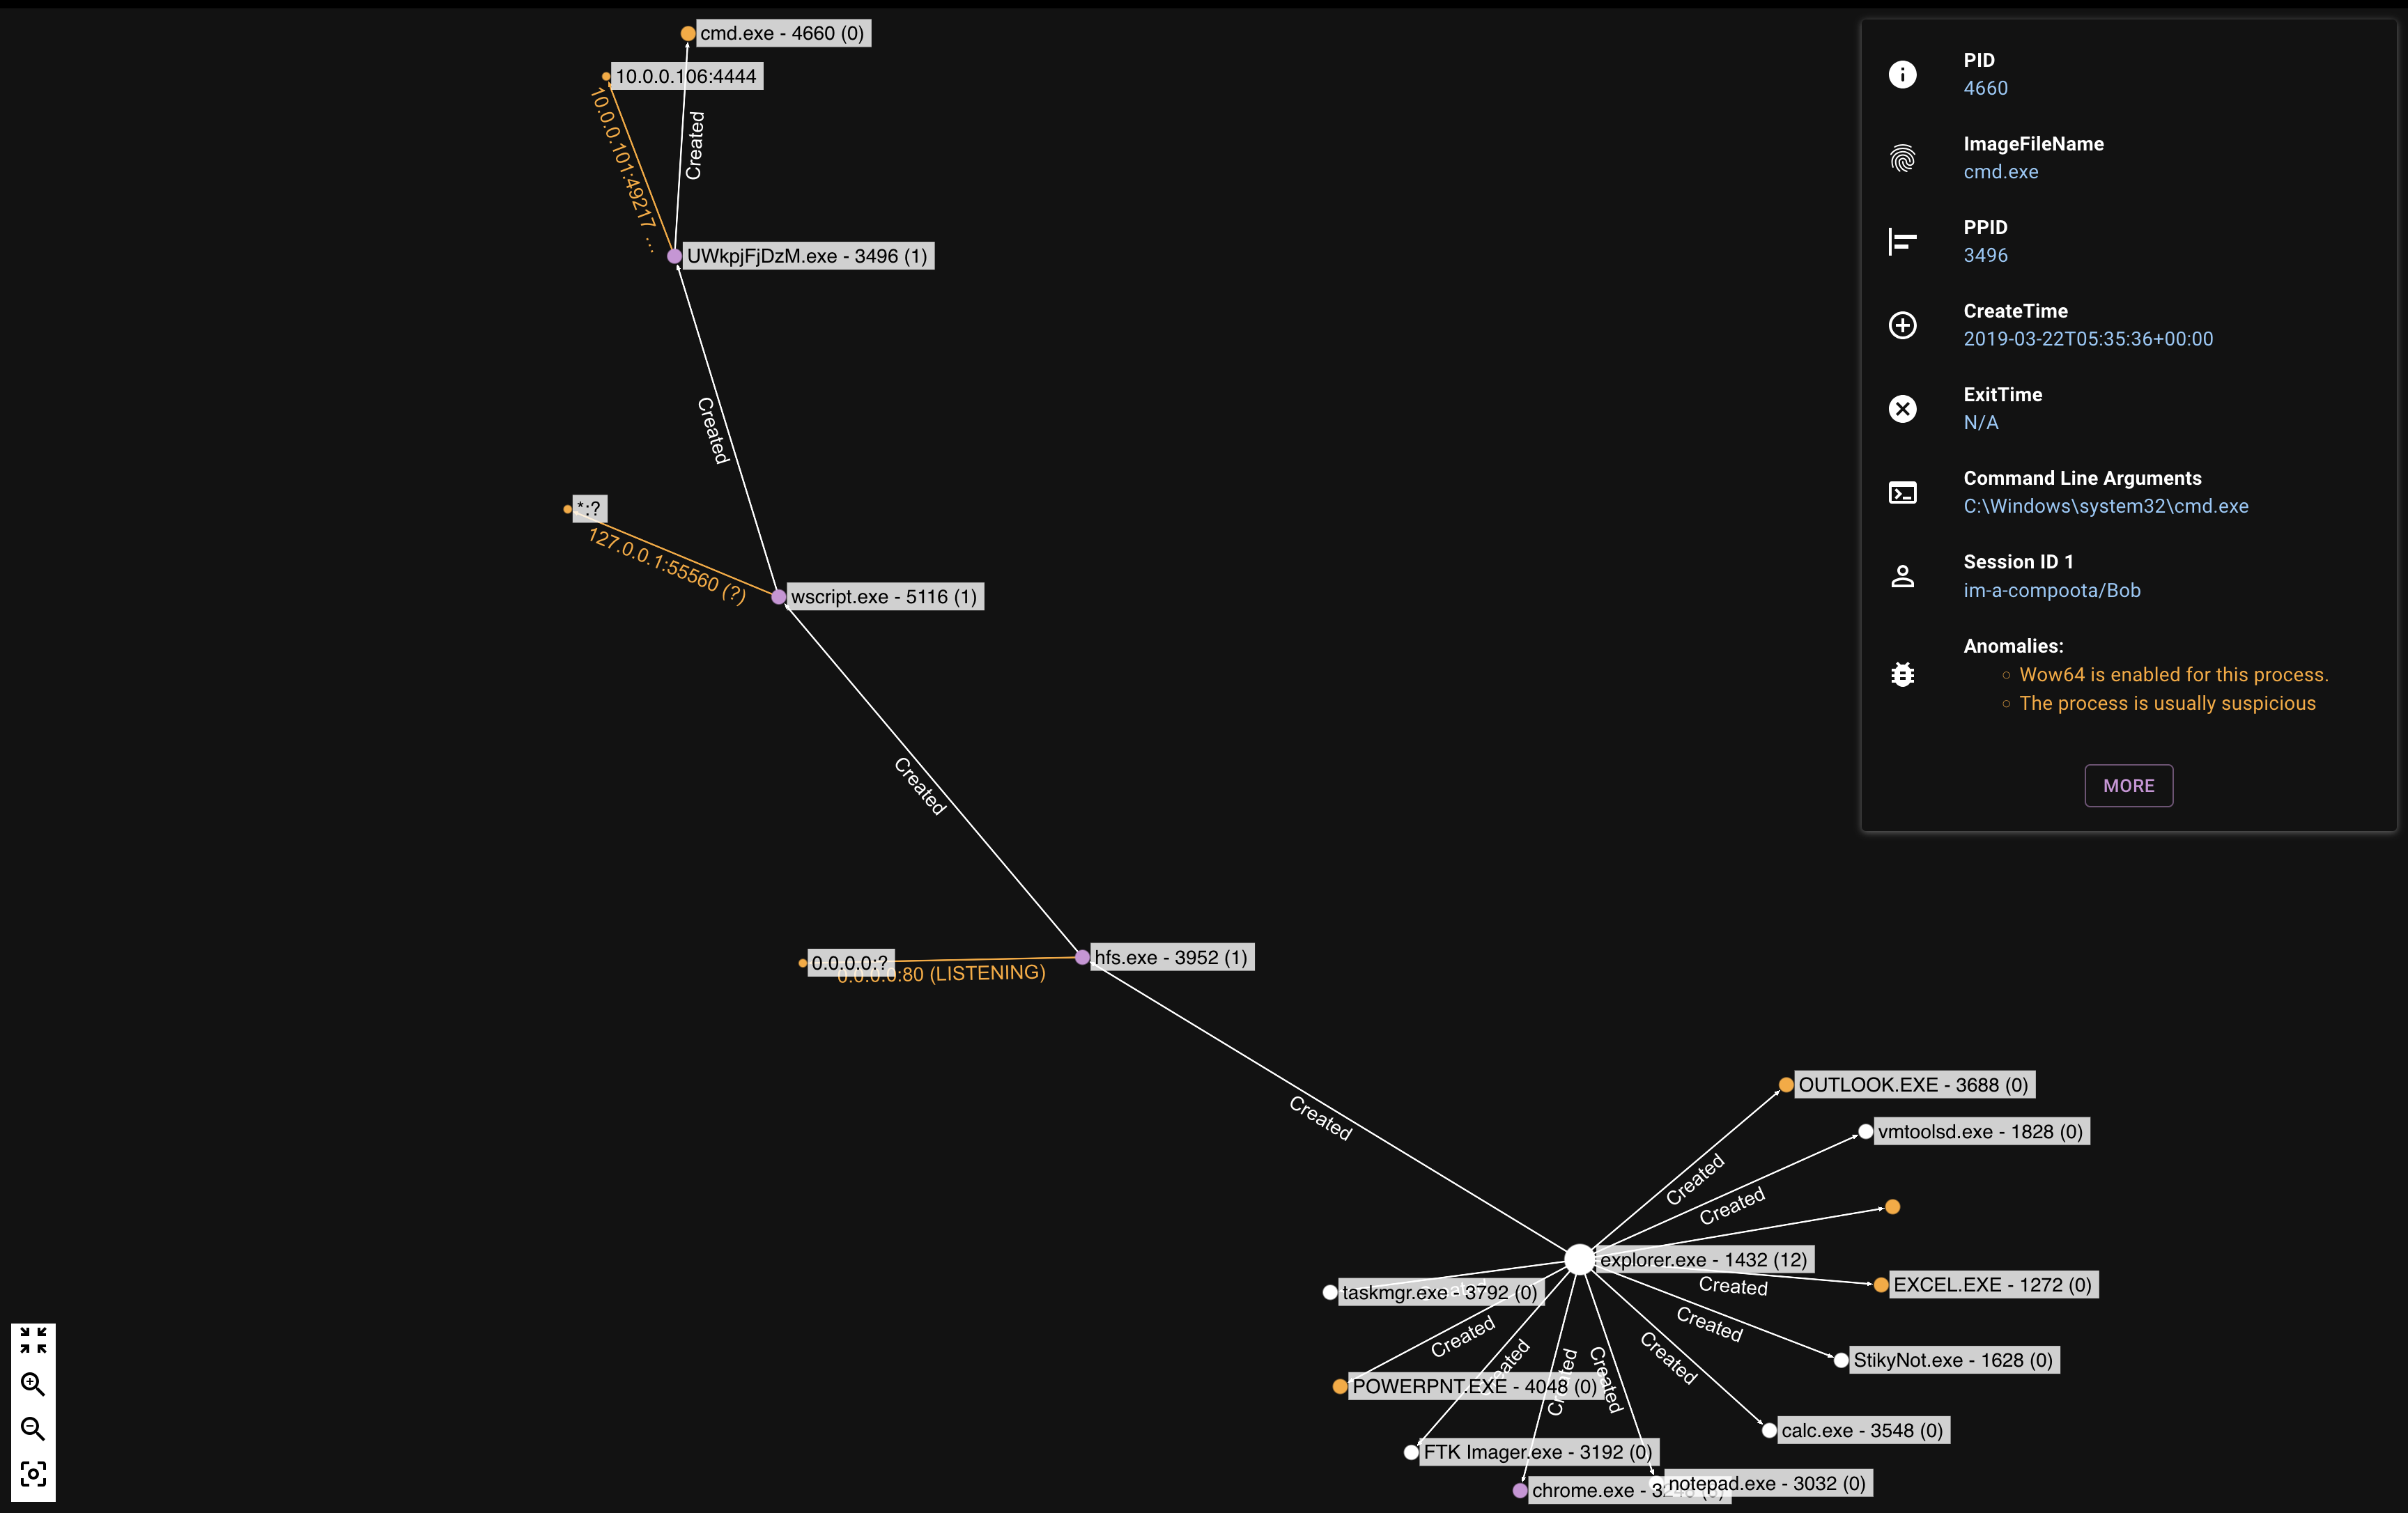
\includegraphics[width=0.9\linewidth]{images/volweb-original/volweb-network-graph.png}
\end{figure}

Le informazioni di rete sono presentate attraverso una combinazione di viste tabellari e visualizzazioni grafiche. La vista tabellare permette un'analisi dettagliata di ogni connessione, mentre la visualizzazione grafica offre una comprensione immediata delle relazioni tra processi e endpoint remoti.

\subsubsection{Sistema di ricerca}

Con dump di memoria che possono contenere informazioni su centinaia di processi e migliaia di artefatti, la capacità di ricerca efficace diventa critica. VolWeb implementa un motore di ricerca che supporta query sia semplici che complesse, permettendo agli analisti di trovare rapidamente informazioni rilevanti. La ricerca full-text opera su tutti i campi dei risultati, permettendo di trovare rapidamente riferimenti a file specifici, indirizzi IP, o stringhe sospette. Il sistema supporta inoltre filtering avanzato per tipo di dato, permettendo per esempio di visualizzare solo i processi che hanno connessioni di rete attive o solo le DLL caricate da percorsi non standard.

\section{Funzionalità Principali}

\subsection{Sistema di Plugin e Estensibilità}

VolWeb implementa un sistema di plugin che riflette e estende quello di Volatility. Ogni plugin supportato è rappresentato da una configurazione che specifica parametri, dipendenze e modalità di visualizzazione dei risultati. Questa architettura permette di aggiungere supporto per nuovi plugin di Volatility senza modifiche al core dell'applicazione.

L'esecuzione dei plugin avviene attraverso Celery task che permettono parallelizzazione e gestione robusta degli errori. Quando un utente richiede l'esecuzione di un'analisi, VolWeb crea un task Celery per ogni plugin selezionato. Questi task vengono distribuiti ai worker disponibili, permettendo l'esecuzione parallela su hardware multi-core o distribuito.

L'orchestrazione dei plugin tiene conto delle dipendenze tra di essi. Alcuni plugin richiedono i risultati di altri per funzionare correttamente. VolWeb gestisce automaticamente queste dipendenze, assicurando che i plugin vengano eseguiti nell'ordine corretto e che i risultati siano disponibili quando necessario.

\subsection{API REST}

VolWeb espone una API REST completa che permette l'automazione e l'integrazione con altri strumenti. La documentazione delle API, generata automaticamente da Django REST Framework, fornisce dettagli su ogni endpoint disponibile, parametri richiesti e formato delle risposte.

\begin{figure}[H]
    \centering
    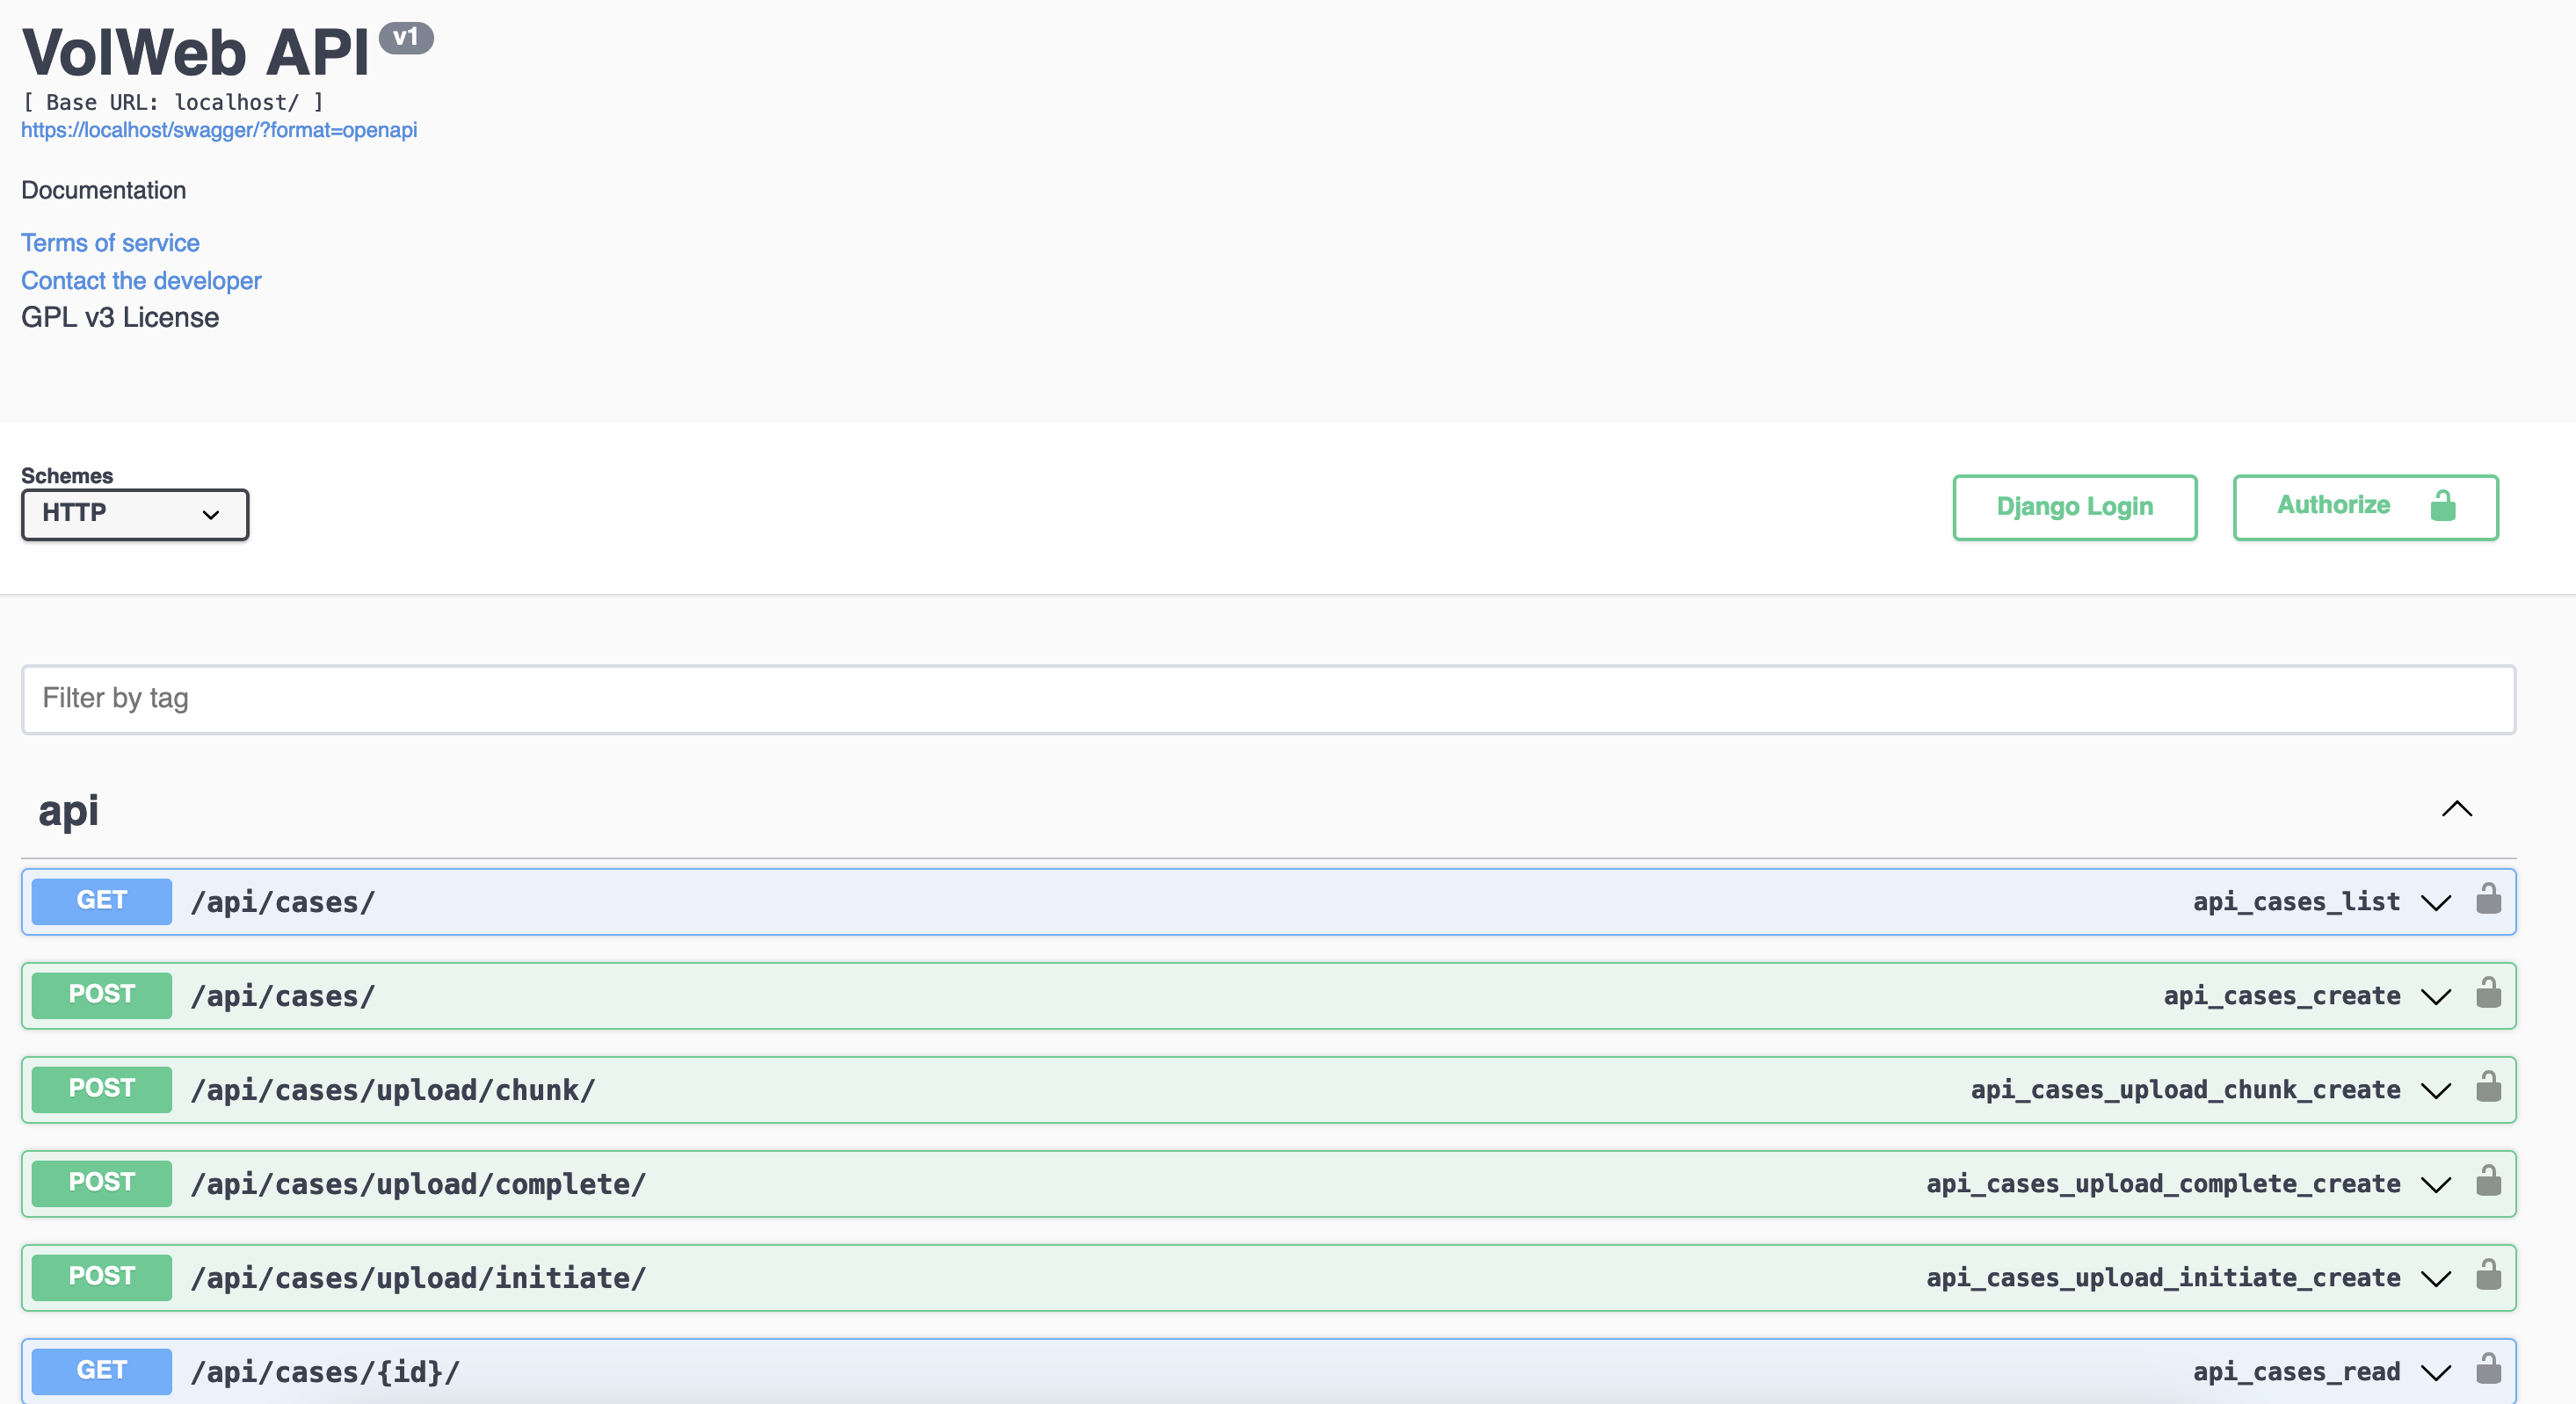
\includegraphics[width=1\linewidth]{images/volweb-original/volweb-swagger.png}
\end{figure}

Gli endpoint principali includono la gestione dei casi con creazione, modifica e cancellazione, la gestione delle evidenze con upload, download e metadata, l'esecuzione dei plugin con selezione, parametrizzazione e monitoraggio, e il recupero dei risultati con filtering, paginazione ed export. Questa esposizione attraverso API standardizzate trasforma VolWeb in un componente integrabile in pipeline di analisi più ampie, permettendo l'automazione di workflow complessi.

\subsection{Sicurezza e Controllo degli Accessi}

La sicurezza in VolWeb è implementata a più livelli, partendo da un robusto sistema di autenticazione basato sul framework di Django. Gli utenti devono autenticarsi per accedere a qualsiasi funzionalità, e le sessioni sono gestite in modo sicuro con token che scadono dopo un periodo di inattività configurabile.

Il sistema di autorizzazione implementa un modello di permessi granulare. Gli utenti possono avere ruoli diversi con capacità appropriate: amministratori con accesso completo, analisti con capacità di creare e gestire casi, e viewer con accesso in sola lettura. A livello di caso, è possibile definire permessi specifici, permettendo la condivisione selettiva di investigazioni tra team diversi mantenendo la segregazione di informazioni sensibili.
\section{Limitazioni e Considerazioni}

Nonostante le capacità significative, la versione originale di VolWeb presenta alcune limitazioni importanti. L'assenza di supporto per YARA rappresenta probabilmente la mancanza più significativa, limitando le capacità di threat hunting della piattaforma. Questa limitazione impedisce l'implementazione di capacità di pattern matching avanzate necessarie per identificare minacce custom o varianti di malware conosciuti, una funzionalità critica in contesti operativi moderni dove le minacce evolvono rapidamente.

Mentre VolWeb presenta i risultati in modo organizzato, manca di capacità avanzate di correlazione tra risultati di plugin che potrebbero identificare automaticamente pattern sospetti attraverso dataset diversi. Questa limitazione richiede che l'analista mantenga mentalmente le correlazioni, aumentando il carico cognitivo durante investigazioni complesse.

L'integrazione con threat intelligence esterna è assente. In un panorama dove la condivisione di IOC e intelligence è fondamentale, l'impossibilità di importare automaticamente feed di threat intelligence o di arricchire i risultati con contesto esterno rappresenta una limitazione operativa significativa. Gli analisti devono manualmente correlare gli artefatti con informazioni esterne, rallentando il processo investigativo.

Nonostante i significativi progressi rappresentati da VolWeb nella democratizzazione dell'accesso alla memory forensics, è stata l'esperienza operativa in contesti ad alta intensità a evidenziare le aree di miglioramento più critiche. Il capitolo seguente analizza come l'esercitazione NATO Locked Shields 2025 abbia fornito il banco di prova ideale per identificare i requisiti che hanno guidato le espansioni presentate in questa tesi.